\documentclass[11pt]{article}

\usepackage{graphicx}
\usepackage{comment}
\usepackage{float}
\usepackage{hyperref}
\usepackage[authoryear]{natbib}
\usepackage{setspace}
\usepackage{mathtools}
%\usepackage{aas_macros}
\usepackage{amssymb}
\usepackage{textcomp}
\usepackage{siunitx}

\title{Acousto-Optical Tunable Filter Atmospheric Imager for Determination of Aerosol Extinction}

\author{Brenden J Elash, Adam E Bourassa, Douglas A Degenstein, Paul(?) }

\begin{document}

\maketitle

\section{Introduction}

The Atmospheric Limb Imager (ALI) is a prototype atmospheric instrument developed at the University of Saskatchewan with the eventual plan for a satellite instrumentation in the future with the purpose to gather high resolution horizontal and vertical aerosol extinction profiles. The purpose of the ALI prototype is to test and verify the use of an Acousto-Optical Tunable Filter (AOTF), the fundamental technology behind ALI, in a space environment and to be gather atmospheric sulfate aerosol profiles with high spacial resolution. ALI will measure light from the atmosphere through the limb geometry which measures the radiance from scattered sunlight from the sunlit atmosphere. ALI is a single channel instrument measuring radiance from the visible to the near infrared wavelengths (650-950~nm) and through successive images build spectral information. The system uses a telescoptic front end to pass collimated light through through the AOTF which is then focused onto the the detector. The AOTF has the unique property of separating the incoming radiance into each of its polarized components selecting one and rotating it polarization through 90 \si{\degree} allowing on to recover some polarization information of the incoming radiance. The ALI prototype was complete in August of 2014 with a stratospheric balloon test flight from the Canadian Space Agency balloon launch facility in Timmins Ontario onboard the CNES gondola platform on September 20, 2014.

\section{Instrument Design}

\subsection{Acouto-Optical Tunable Filter}

Start with background of AOTF theory (momentum matching etc) then Cover the rational for picking the wavelength range that was used for the AOTF as well the the significance of the testing results.

\subsection{Optical Design and Performances}

Outline optical layout and rational for picking it with regard to aerosol concentrations optical characteristics. Final results and expected resolutions and wavelength

\section{Stratospheric Balloon Flight}

\subsection{Flight Day Conditions and Flight Path}

As the title says

\subsection{Measurements}

How measurements are made. Processing from level 0 -> level 1

\subsection{Retrievals}

The method on how the retrievals are transferred from level 1 data to aerosol profiles (level 2). (MART method with OMPS algorithm for particle size)

\subsection{results}

What the final measurements showed and how they compare to SOLAMON and OSIRIS

\section{Conclusions and Future Prospects}

Self explanatory.

Figure for Measurement and retrieval section not completed yet.

\begin{figure}[h!]
    \begin{center}
    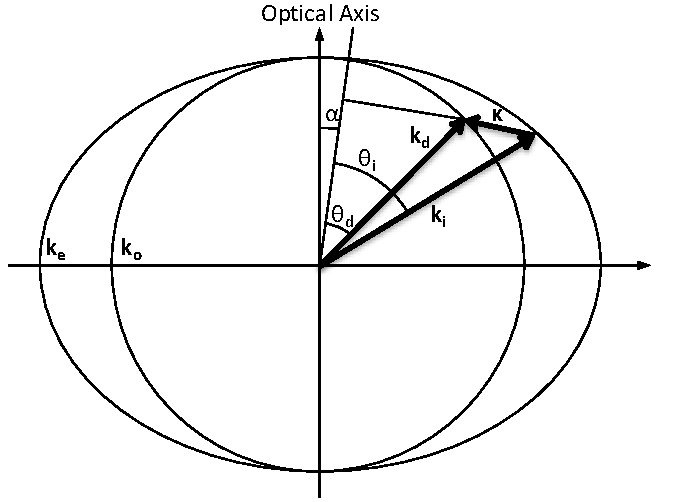
\includegraphics[width=0.7\textwidth]{./Images/3-1-AOTFWavevectorWithRefraction.pdf}
    \caption[Wave Vectors Generated by an AOTF]{The wave vectors generated by the AOTF experiment set up in \autoref{fig:3.1:AOTFExperimentalSetUp}. From the above figure $k_{e}$ and $k_{o}$ are the wave vectors of the extraordinary and ordinary axis of the AOTF crystal and can be represented as $2\pi n_{e}/\lambda$ and $2\pi n_{o}/\lambda$ respectively. The cut angel, $\alpha$, is the cut angle form the optional axis to the piezoelectric transducer.}
    \label{fig:3.1:ATOFWavevectors}
    \end{center}
\end{figure}

\begin{figure}[h!]
    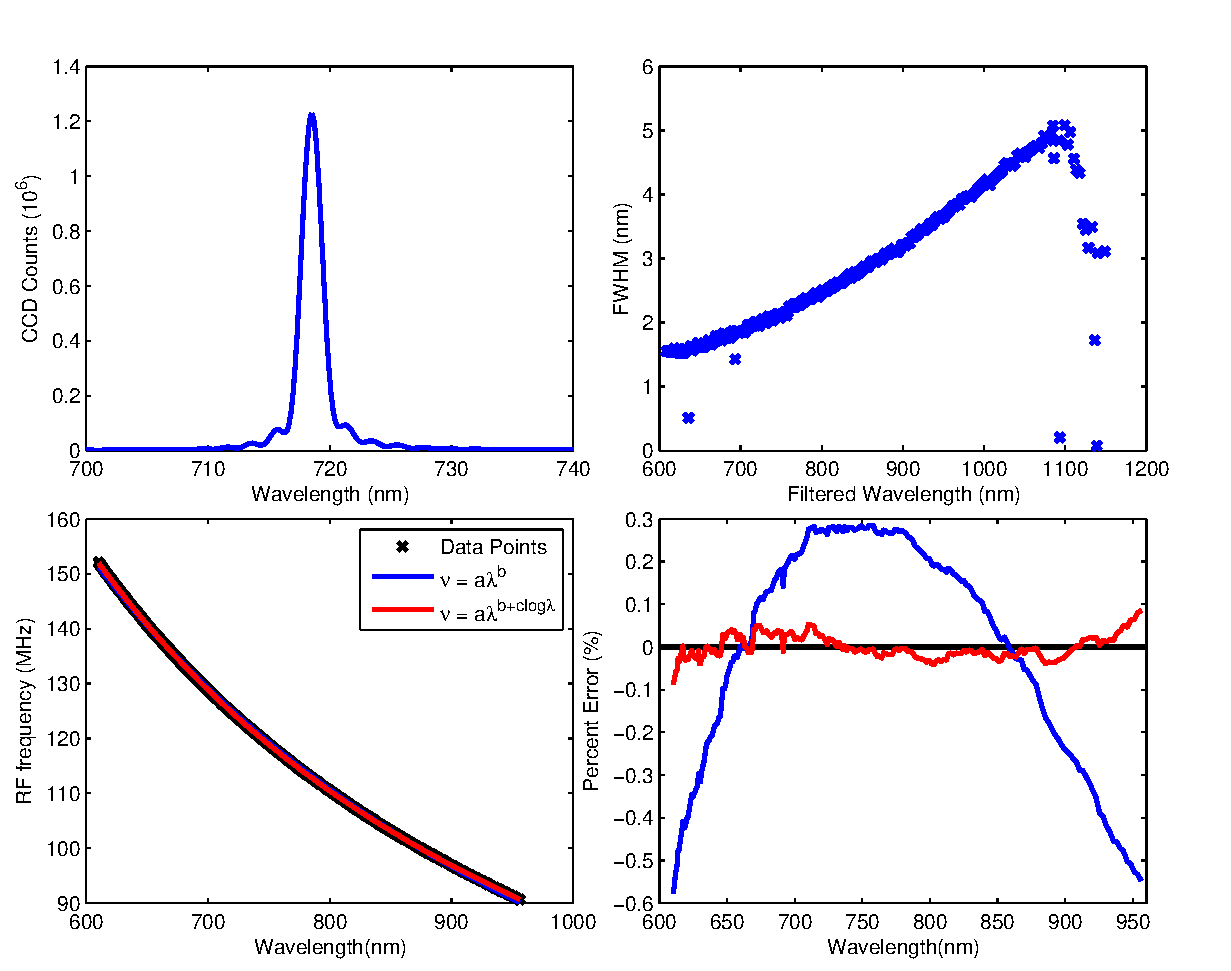
\includegraphics[width=1.0\textwidth]{./Images/3-1-AOTFCharaterization.pdf}
    \caption[Characterization Curves for the Brimrose AOTF]{Top Left: A standard image taken from the AOTF calibration experiment when the tuning frequency of the AOTF was at 124.96~MHz. Top Right: The FWHM for each of the determined wavelengths for the AOTF. It should be noted that the FWHM at 600~nm is 1.5~and as the wavelengths get longer the FWHM increases to 4.9 at 1080~nm. Bottom Left: The calibration curves for the AOTF RF versus the  diffracted wavelength which contains the data points recorded and two best fit curves. Bottom Right: The percent error with respect to the measured frequency for the two best fit curves in the previous panel. It can be noted the modified power function approximates the AOTF wavelength dependance to within 0.1\%.}
    \label{fig:3.1:AOTFCharaterization}
\end{figure}

\begin{figure}[h!]
    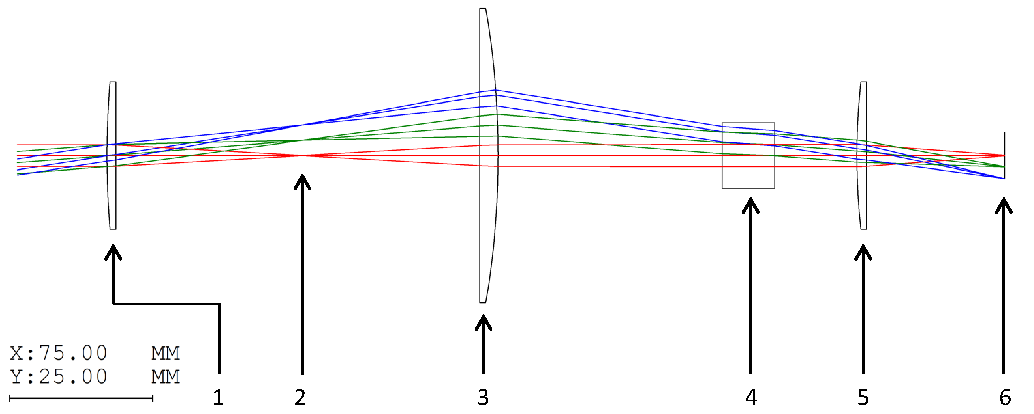
\includegraphics[width=1.0\textwidth]{./Images/3-2-TelescopicRayTracing.pdf}
    \caption[ALI Telescopic Design Prototype]{Ray Tracing diagram of the telescopic lens system simulated by Code V. The elements in the system are the following: (1) 100~mm focal length plano-convex lens. (2) Location where shutter will be located to limit stray light (3) 100~mm focal length plano-convex lens. (4) Brimrose AOTF characterized in \autoref{sec:3.1:AOTFCalibration}. (5) 75.6~mm focal length plano-convex lens. (6) Imaging plane. It should be noted that the x and y scales are not the same in this image. Also, in the lab a polarizer is added in front and behind the AOTF as well as prisms behind the AOTF.}
    \label{fig:3.2:telescopicRayTracing}
\end{figure}

\end{document} 